% Methods
In this chapter, a description of event selection is given, as well as definitions of
key physical variables and how they are used to select events. Then, a procedure regarding
how the signal sample is manipulated to produce a high statistics off-shell tail is described.
Finally, the binning of variables used to obtain the results is determined and defined.

\section{Event selection and physical variables}
\begin{itemize}
    \item Description of homebrew event variables and their physical significance
    \item DJJ\_VBF prescription
\end{itemize}
Proton bunches cross each at a rate of about \SI{400}{\mega\hertz} in the beam line of
the LHC, naturally, not all of these crossings are recorded due to both technical
limitation of the electronics as well as the fact that the vast majority of these
crossings don't produce inelastic collision that is energetic enough to be interesting to us.

After the selection of Level 1 (L1) trigger and the higher level trigger (HLT), less than 1000
events per second are permanently recorded and would go to off-line, full reconstruction. Among these,
we only select the ones that passes certain triggers.
\todo[inline]{give a correct account for what trigger is used for 2018}

After selecting mandating passing certain triggers, we make a base line cut in the variables
based on more delicate physics reason, the list of base line cuts is as below:
\begin{itemize}
    \item No ak4-jet b-tagged jet
    \item Both leptons have $p_\mathrm{T} > \SI{25}{\giga\electronvolt}$
    \item $\abs{\Delta\phi_{\ell\ell\_\met}} > 1.0$
    \item $\abs{\Delta\phi_{\ell\ell\mathrm{Jet}\_\met}} > 2.5$
    \item $\abs{m_{\ell\ell} - 91.2\gev} > 15\gev$
    \item $p_\mathrm{T}^{\ell\ell} > 55\gev$
    \item $\met > 125\gev$
    \item min($\abs{ \Delta\phi_{\mathrm{j}\_\met}}$) < 0.25
\end{itemize}
\todo[inline]{define the uncommon ones and give account for the choice}
\missingfigure{Show how much backgrounds are gone for maybe 2 samples}
\newpage\phantom{blabla}

\section{Backgrounds}
\begin{itemize}
    \item Remarks on a few `fakeable' physical objects
    \item a interference background in Higgs sample
\end{itemize}
\missingfigure{base plots for varibles, stress ones with discriminative power}
\newpage\phantom{blabla}


\section{Signal simulation reweighting}
\begin{itemize}
    \item Physics of Higgs signal sample (the weight, ME)
    \item the need for pieceing together samples with different LHE Mass
    \item results (also see appendix A)
\end{itemize}
\begin{figure}[htb]
\begin{center}
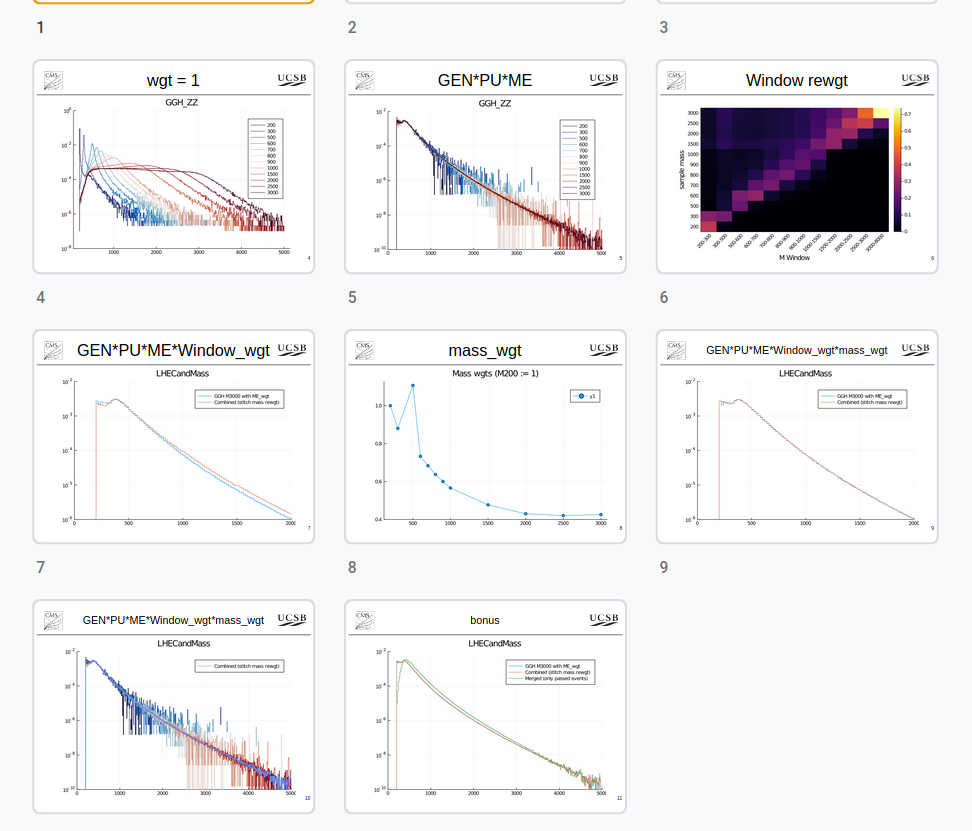
\includegraphics[width=.90\linewidth]{fig/signal_rewgt_placeholder.png}
\end{center}
\label{fig:sig_rewgt}
\end{figure}
\todo[inline]{describe these steps}
\newpage\phantom{blabla}


\section{Strategy in variable selection and binning}
\begin{figure}[htb]
\begin{center}
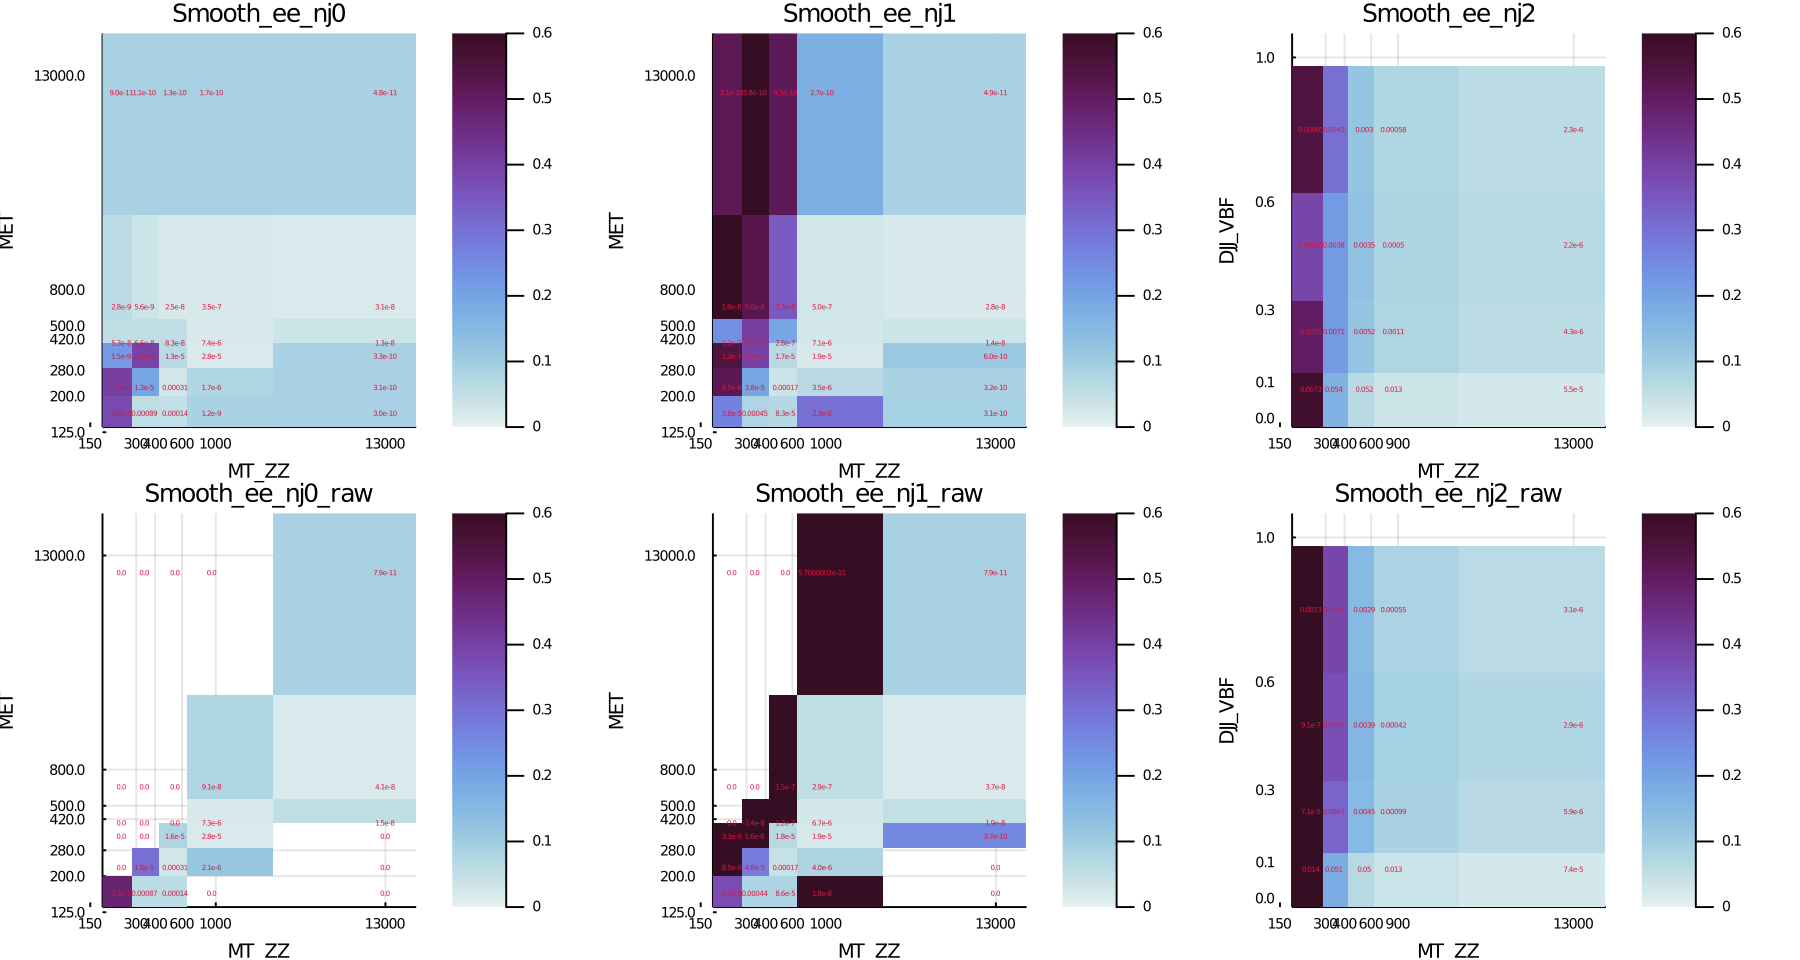
\includegraphics[width=.90\linewidth]{fig/binning_placeholder.png}
\end{center}
\label{fig:sig_rewgt}
\end{figure}
\todo[inline]{make plots publication quality and give quantitative justification for choice}
